\section{static libraries}


\subsection{Wozu?}

\begin{frame}{Woher kommt C++?}
	C++ versucht, ein Hansdampf in allen Gassen zu sein, also:
	
	\begin{itemize}
		\item Effizient, schnell
		\item flexibel: für alle Plattformen
		\item flexibel: für alle Aufgaben
		\item flexibel: für n+1 Wege, etwas zu tun
	\end{itemize}
	
	\pause
	\vspace{1em}
	
	\alert{ Resultat: Eine riesige und komplexe Sprache, die auf dem \emph{kleinsten gemeinsamen Nenner} definiert ist. }
\end{frame}

\begin{frame}[fragile]{Was ist C++?}
	C++ ist eine standardisierte Programmiersprache. Wir arbeiten mit dem (veralteten) ISO/IEC 14882:2003
	
	\vspace{1em}
	
	Der Standard beschreibt grob:
	\begin{itemize}
		\item Erzeugung von Quellcode (Präprozessor, Templates)
		\item was gültiger Quellcode ist
		\item das beobachtbare Verhalten eines Programms
	\end{itemize}
	
	\pause
	\vspace{1em}
	
	\begin{block}{Beobachtbares Verhalten}
		\begin{itemize}
			\item Speicherzugriff auf als \verb|volatile| markierte Daten
			\item I/O-Funktionen der (Standard-)Bibliothek
		\end{itemize}
	\end{block}
\end{frame}

\begin{frame}[fragile]{Was kann C++?}
	\begin{block}{Speicherzugriff}
		\begin{itemize}
			\item Berechnungen, Prüfungen usw.
			\item Kopien an bestimmte Orte
		\end{itemize}
	\end{block}
	
	\pause
	\vspace{2em}
	
	\begin{block}{I/O-Funktionen}
		\begin{itemize}
			\item Zeichenweise Ein-/Ausgabe (\verb|cin|, \verb|cout|) ABER keine Konsole/Shell
			\item Zugriff auf Dateien (\verb|ofstream|, \verb|ifstream|) ABER keine Ordnerstruktur
		\end{itemize}
	\end{block}
\end{frame}

\begin{frame}{Programm-Bibliotheken}
	Programm-Bibliotheken enthalten code (Anweisungen) und/oder Programmierhilfen.

	\vspace{2em}
	
	Szenarien für Programm-Bibliotheken:
	\begin{itemize}
		\item Modularisierung des eigenen Programms
		\item gebräuchliche Funktionalitäten (z.B. Ringpuffer)
		\item Abstraktion / Verstecken von Implementierung (z.B. SDL, qt)
		\item Verringerung der build-Dauer
	\end{itemize}
\end{frame}

\begin{frame}{Mehr Funktionalität durch Bibliothek}
	\begin{itemize}[<+->]
		\item Der Compiler kennt die target platform (z.B. Linux auf x64)!
		\item Compiler-spezifische Anweisungen können in Plattform-abhängige Befehle übersetzt werden
		\item bestimme Anweisungen für Kommunikation mit Hardware oder Betriebssystem
	\end{itemize}
	
	\vspace{2em}
	\uncover<+->
	{
		Entweder: die Compiler-spezifischen Anweisungen direkt in den Quellcode\\
		Oder: \uncover<+->{ \alert{ diese Anweisungen in Bibliotheken verstecken } }
	}
\end{frame}

\begin{frame}{Beispiele für verschiedene Bibliotheken}
	\begin{block}{Modularisierung}
		\begin{itemize}
			\item Bitmap-Framework als static library
			\item cuviso device com libs
		\end{itemize}
	\end{block}
	
	\pause
	\vspace{0.5em}
	
	\begin{block}{Gebräuchliche Funktionalitäten}
		\begin{itemize}
			\item Boost.Math, Boost.Algorithm, Boost.Container (header-only!)
			\item FFT-Bibliotheken
		\end{itemize}
	\end{block}
	
	\pause
	\vspace{0.5em}
	
	\begin{block}{Abstraktion von der Implementierung}
		\begin{itemize}
			\item Standard-I/O-Bibliotheken
			\item pthreads, Boost.Thread
			\item qt (mehr als nur eine lib)
			\item Windows SDK (mehr als nur eine lib)
		\end{itemize}
	\end{block}
\end{frame}


\subsection{statically linked libraries}

\begin{frame}{Zusammenspiel mit dem Programm}
	\alt<1>
	{% on slide 1
		\includegraphics[width=\textwidth]{images/translation}
	}{% on all other slides
		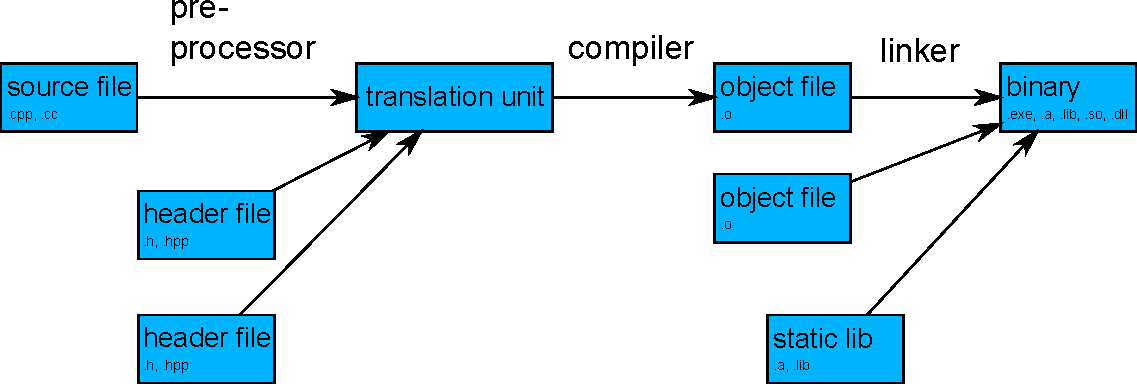
\includegraphics[width=\textwidth]{images/translation-lib}
	}
	
	\vspace{2em}
	\uncover<3->
	{
		\begin{block}{Terminologie}
			\emph{statically linked program library}, kurz \emph{static library}
			
			Eine vom Linker während des build-Vorgangs fest eingebaute Bibliothek.
		\end{block}
	}
\end{frame}

\begin{frame}{Zusammenspiel mit C++}
	\alert{ C++ selbst bietet keinerlei Unterstützung für static libraries }
	
	\uncover<+->
	
	\begin{itemize}[<+->]
		\item Wie auch schon das Mitteilen, welche object files der Linker verarbeiten soll, ist die Verwendung von static libraries abhängig vom verwendeten Linker.
		\item Zumeist werden static libraries wie vorkompilierte object files behandelt, es gelten also dieselben linkage-Regeln.
		\item Header-Files zu static libraries ermöglichen den Zugriff im Programm auf Namen in der Bibliothek mit external linkage.
	\end{itemize}
	
	\uncover<+->
	{
		Eine static library lässt sich
		\begin{itemize}
			\item schreiben wie \enquote{ein Programm ohne main}
			\item nutzen wie ein weiterer Header (compiling) und wie eine weitere object file (linking)
		\end{itemize}
	}
	
	\uncover<+->
	{
		\alert{ Aber: Gott tötet kleine Kätzchen wenn man einfach Programm X nimmt, die main weglässt, und das eine Bibliothek nennt. }
	}
\end{frame}

\begin{frame}[fragile]{Verwendung von static libs (cmd-line)}
	\footnotesize
	
	\begin{block}{Übliche cmd-line-Parameter}
		\begin{itemize}
			\item Kompilieren: \verb|compile program.cpp -o program.o| \\
			\item Linken (1): \verb|link program.o myLib.a -o program| \\
			\item Linken (2): \verb|link program.o -lmyLib -o program|
		\end{itemize}
	\end{block}
	
	\pause
	
	\begin{block}{Vereinfachung: library search paths}
		\begin{itemize}
			\item Libraries sind zumeist in sich abgeschlossen, und daher prädestiniert für einen eigenen Ordner.
			\item Libraries für gebräuchliche Funktionalitäten sind prädestiniert für Projekt-unabhängige Orte/Ordner.
		\end{itemize}
		
		\pause
		
		\emph{include search path:} Pfad, von wo aus der Compiler nach {\tiny \verb|#include <path/file.ext>| } sucht \\
		Angabe durch Parameter: \verb|compile -I"include_search_path"|
		
		\pause
		\vspace{0.5em}
		
		\emph{library search path:} Pfad, wo der Linker eine Bibliothek sucht \\
		Angabe durch Parameter: \verb|link -L"lib_search_path"|
	\end{block}
\end{frame}

\begin{frame}{Verwendung von static libs (IDE)}
	\begin{itemize}[<+->]
		\item In IDEs gibt es üblicherweise GUIs zur Konfiguration der cmd-line-Parameter von Compiler und Linker.
		\item Im speziellen: Verwaltung von static libs
		\item Je nach IDE an unterschiedlicher Stelle und mit unterschiedlicher Mächtigkeit
		\item \alert{ Manuell die Pfade {\tiny (include search path, library search path) } anzugeben ist eine \emph{sehr} rudimentäre Methode, aufwändig und fehleranfällig. }
	\end{itemize}
	
	\vspace{2em}
	
	\uncover<+->
	{
		Fazit: Am Ende sind es cmd-line-Parameter von Compiler und Linker, man kann sie auf unterschiedlichen Wegen setzen.
	}
\end{frame}

\begin{frame}[fragile]{Hinweise zur Verwendung}
	\begin{itemize}[<+->]
		\item üblicherweise werden static libraries in Ordner gegliedert: \\
		\verb|mylib/inc| $\rightarrow$ include search path \\
		\verb|mylib/lib| $\rightarrow$ library search path
		\item library header (\verb|.h|) $\rightarrow$ Compiler \\
		library file (\verb|.a|, \verb|.lib|) $\rightarrow$ Linker
		\item (precompiled) static libraries sind Compiler-, Linker- und Plattform-abhängig! Auch mglw. von deren Version!
		\item static libraries erhält man vorwiegend aus dem Internet/www, unter Linux auch über die Paketverwaltung
		\item manche static libraries (z.B. SDL) binden intern (versteckt) eine DLL / ein SO ein $\implies$ achte auf Abhängigkeiten!
	\end{itemize}
\end{frame}



